\section{Codificação das instruções}
	Instrução é uma palavra da linguagem de máquina, sua codificação é de fundamental importância para o processamento das operações.	 
  	\\Todas as instruções contém 32 bits. Exitem 4 formatos de instruções: R (R-type), I (I-type), Load/Store e Jump.
  	\\O formato R está relacionado as instruções lógicas e aritméticas.
	\begin{figure}[H]
    	\centering
    	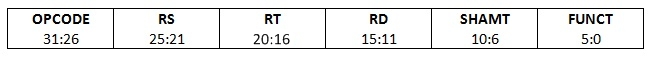
\includegraphics{r-format}
    	\caption{Formato R}
		\label{r_format}
	\end{figure}
	Seus respectivos campos são:
	\begin{itemize}
	\item \textbf{OPCODE} - Código da operação básica da instrução.
	\item \textbf{RS} - Registrador do primeiro operando de origem.
	\item \textbf{RT} - Registrador do segundo operando de origem.
	\item \textbf{RD} - Registrador destino.
	\item \textbf{SHAMT} - \textit{Shift amount}; Quantidade de deslocamento.
	\item \textbf{FUNCT} - Função; Esse campo seleciona a variante específica da operação no campo opcode, e as vezes, é chamado de código de função.
\end{itemize}	  	
  	Um segundo tipo de formato de instrução é chamado de formato I, utilizado pelas instruções imediatas e de transferência de dados.
	\begin{figure}[H]
    	\centering
    	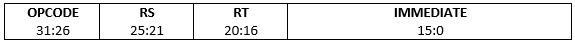
\includegraphics{i-format}
    	\caption{Formato I}
		\label{i_format}
  	\end{figure}
Seus respectivos campos são:
	\begin{itemize}
	\item \textbf{OPCODE} - Código da operação básica da instrução.
	\item \textbf{RS} - Registrador do operando de origem.
	\item \textbf{RT} - Registrador destino.
	\item \textbf{ADDRESS} - Endereço de memória ou constante numérica.
\end{itemize}	  	
  	
  	\begin{figure}[H]
    	\centering
    	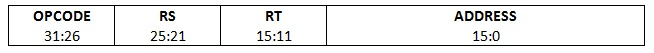
\includegraphics{load-store}
    	\caption{Formato Load/Store}
		\label{loadstore}
  	\end{figure}
  	
   	\begin{figure}[H]
    	\centering
    	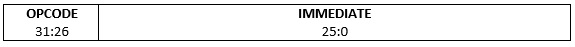
\includegraphics{jump}
    	\caption{Formato Jump}
		\label{jump}
  	\end{figure}
  	
 